\chapter{State of the art}

    This chapter aims to provide a literature overview to the topics that relate to the main problem that this thesis aims to help solve, which is the lack of cooperation between applications and the infrastructure where they reside.
    As such, the first section focuses on discussing structural network patterns utilized by applications to give them particular properties which are helpful to achieve their use case.
    Among these patterns, particular interest will be given to three of them for the following reasons: firstly, due to their popularity in the current network paradigm; secondly, due to their potential to optimize traffic which is generated at the application level.
    These patterns are thus the classical server-client architecture, the distributed approach of peer-to-peer (P2P) architectures, and content distribution networks (CDNs).
    For each of these, a conceptual analysis is made - more specifically, contextual background, the architecture itself, advantages and disadvantages, and possible use cases.
    Additionally, there's an examination on how applications that utilize these networks affect, positively or negatively, the physical infrastructure where they operate on, and where does potential reside for mutually-beneficial cooperative behaviour between these two layers.
    The following section displays existing proposals for increased layer cooperation, and alongside it a discussion on the practical consequences of adopting such proposals.
    The final chapter gives special attention to the Application-Layer Traffic Optimization (ALTO) working group's proposal, as it is the baseline for this thesis's work..

\section{Peer-to-Peer (P2P) Networks}

\subsection{Concepts and Applications}

    Due to the many hybrid implementations that have surfaced, the definition of a P2P network has become harder to pinpoint.
    Nevertheless, a P2P network is grounded on some definitions, among them that it consists on many singular computing elements, the "peers", which have among themselves similar privileges and functions (this contrasts with the client-server architecture, where two different roles exist - the one that provides a service and the one that can consume it - with functionality and control being thus centralized).
    P2P networks decentralize computational resources as a means to achieve a given task in a way that is inherently different to a centralized counterpart.
    This decentralized architecture of the entire system as a whole gives it an interesting list of properties, among them:

\begin{itemize}
    \item \textbf{Dynamic scaling}: As all member nodes can share their computing resources with the network, the system increases its capacity with an increase in its users.
        Since the peers also act as clients to the network, scaling the service becomes less of a challenge as each new client will also act as a server.
        This also removes the necessity to manage how many service resources are needed - the amount of existing resources is linked to the number of existing clients, and thus there's no need to purchase and manage central resources, as the network dynamically allocates them by nature.
    \item \textbf{Resilience to failure}: Whereas centralized solutions are vulnerable to node and link failure, a decentralized one can more easily work around such threats - as all peers can encompass the same server functionality, network services and resources are not provided on a limited set on nodes, but instead can be redundantly deployed throughout as needed.
    \item \textbf{Power decentralization}: As a direct consequence of the sharing resources, no single peer has direct control of the network, and the information is not centralized.
        As such, this considerably deters any attempts to overpower the network, e.g., via means of censorship or biased node favouring.
\end{itemize}

    These, however, are not without their nuances - since many P2P hybrids exist, these properties are not immutable.
    For example, if we consider BitTorrent, which has Tracker servers to redirect users to a correct peer with the requested resource, whilst the network itself can still be resilient to failure, the content-retrieval service that the P2P network provides has a single point of failure and of control - the trackers themselves.
    Furthermore, the P2P network design brings, by its nature, alongside their potentially advantageous properties, also some some potentially disadvantageous ones to consider:

\begin{itemize}
    \item \textbf{Security hazards:} The equal functionality property that P2P networks have give peers much power influence others.
        Without proper care, malicious peers are a security risk.
    \item \textbf{Management:} Since resources and services are not centralized, tasks such as event logging and resource backups become very difficult, and perhaps impossible if the peers do not abide by any proper orchestration strategy.
\end{itemize}

    P2P applications have had, in the past decades, a mainstream image that is plagued with legality and security issues.
    Nonetheless, when overcome, the P2P networking strategy possesses many interesting properties - some of them displayed above - that make it fitting for varied use cases, e.g., file sharing, media streaming, social networking and problem solving via distributed and cooperative algorithms.

    Either way, the influence of P2P applications is undeniable: Sandvine's global Internet phenomena report concluded that BitTorrent alone had in 2019 a global application total traffic share of 2.4\%, and perhaps most importantly over 27\% of total upstream volume of traffic, and over 44\% in Europe, the Middle East and Africa (EMEA) alone \cite{sandvine2019}.
    Beyond file sharing purposes alone, P2P applications have been recently considered a fitting solution for low-cost content delivery systems in high demand scenarios - for example,  in applications such as PPStream in China which provide television content over IP to large audiences.
    Similarly, Akamai recognizes the potential of P2P technologies to provide a highly distributed option for serving static content over the network, although it being currently lacking in management and control features \cite{akamai-report}.
    Indeed, peer-to-peer Internet video broadcast services - and world-wide static content delivery services for that matter - seem attractive as they are cost-effective and easy to deploy, and are fitting to larger scale demands, and thus have the potential to become a more mainstream solution \cite{jianchuanliu2008}.

    Concluding, the P2P network architecture has many fitting use cases, and their rather different strategy, compared to the client-server architecture, to achieve its goals gives it many potentially interesting properties for users and ISPs.
    Considering its large global traffic share, particularly in upstream traffic, and its potential adoption towards the large scale demands of the future, P2P applications are likely to persist in the future and will be in the minds of ISP administrators.

\subsection{Architecture}

    As stated previously, the term "Peer-to-peer" has become very broad and now serves as an umbrella for many different variations of the core decentralized architecture.
    Thus, this chapter focuses not on overviewing a single conceptual architecture of what defines a P2P network, but instead of the many existing variations and how they differ among themselves.
    All P2P networks are characterized by consisting of peers that know one another as to form a so-called overlay network on top of its supporting network.
    How peers are organized in these P2P networks and how they operate is what distinguishes the many sub-types.
    Table \ref{table:p2p-structures} groups known P2P systems in regards to their centralization and structure, as did \cite{p2p-survey-1} and \cite{p2p-survey-2}, with the latter further distinguishing the protocols in regards to other metrics, e.g., security, reliability, and performance.
    The rest of this section follows the survey made by the former.


    One would expect that all P2P applications would have no centralization at all, since the P2P design ponders  spread throughout the network.
    However, some modifications have been made in some of these sub-types, which shift how much decentralization they have.
    Similarly, different strategies exist that dictate the structural hierarchy of the peers on the network.
    As would be expected, these sub-types of P2P networks thus possess different strengths and weaknesses, and these can be leveraged to the most appropriate use cases.

\begin{table}[]
\caption{Types of P2P systems (Adapted from \cite{p2p-survey-1})}
\label{table:p2p-structures}
\begin{adjustbox}{max width =1.1\textwidth,center}
\begin{tabular}{lllllll}
                                                 &                                        &                                                                                 &                                                                                                                 &                                                                                                                          &  &  \\ \cline{3-5}
                                                 & \multicolumn{1}{l|}{}                  & \multicolumn{3}{c|}{Centralization}                                                                                                                                                                                                                                                                                          &  &  \\ \cline{3-5}
                                                 & \multicolumn{1}{l|}{}                  & \multicolumn{1}{l|}{Hybrid}                                                     & \multicolumn{1}{l|}{Partial}                                                                                    & \multicolumn{1}{l|}{None}                                                                                                &  &  \\ \cline{1-5}
\multicolumn{1}{|c|}{\multirow{9}{*}{Structure}} & \multicolumn{1}{l|}{None}              & \multicolumn{1}{l|}{\begin{tabular}[c]{@{}l@{}}Bittorrent, Napster,\\ Publius\end{tabular}} & \multicolumn{1}{l|}{\begin{tabular}[c]{@{}l@{}}Kazaa,\\ Morpheus,\\ Gnutella (extension proposals),\\ Edutella\end{tabular}} & \multicolumn{1}{l|}{\begin{tabular}[c]{@{}l@{}}Gnutella,\\ FreeHaven\end{tabular}}                            &  &  \\ \cline{2-5}
\multicolumn{1}{|c|}{}                           & \multicolumn{1}{l|}{In Infrastructure} & \multicolumn{1}{l|}{}                                                           & \multicolumn{1}{l|}{}                                                                                           & \multicolumn{1}{l|}{\begin{tabular}[c]{@{}l@{}}Chord,\\ CAN,\\ Tapestry,\\ Pastry\end{tabular}}                          &  &  \\ \cline{2-5}
\multicolumn{1}{|c|}{}                           & \multicolumn{1}{l|}{In System}         & \multicolumn{1}{l|}{}                                                           & \multicolumn{1}{l|}{}                                                                                           & \multicolumn{1}{l|}{\begin{tabular}[c]{@{}l@{}}Bittorrent (DHT/Trackerless), \\OceanStore,\\ Mnemosyne,\\ Scan, PAST,\\ Kademlia,\\ Tarzan\end{tabular}} &  &  \\ \cline{1-5}
                                                 &                                        &                                                                                 &                                                                                                                 &                                                                                                                          &  &
\end{tabular}
\end{adjustbox}
\end{table}

    Early versions of Gnutella come as a famous example of a decentralized and unstructured architecture, as peers act with equal functions and privileges, and no inherent structure exists on how these peers connect to others, nor does it on storing or retrieving content on the network.
    The bootstrapping method consists on users reading from a set of known Gnutella peers, which is essentially a static list of addresses obtained from a trustworthy source, and attempting to connect to each one of them until a preferred number of known neighbours is reached.
    The unstructured nature of this protocol makes it so there's no systematic way to efficiently retrieve content, as thus peers must flood the network with content queries until either a reply is met or the predefined TTL value is exceeded, as can be seen on Figure \ref{fig:gnutella-flood}.

\todo{reference gnutella-flood.png}

\begin{figure}[!h]
\centering
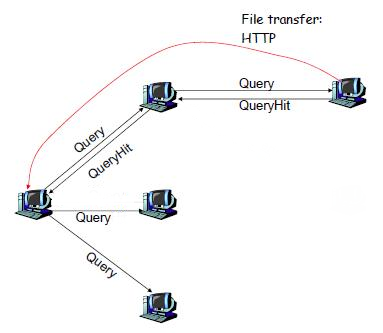
\includegraphics[scale=1.2]{img/gnutella-flood.png}
\caption{Demonstration of Gnutella's file searching mechanism \cite{p2p-survey-1}}
\label{fig:gnutella-flood}
\end{figure}

    Partially centralized architectures were defined as similar to those which are decentralized, but with the added caveat that some peers are chosen to service a portion of the network.
    This is done to take use from the fact that not all network peers are alike in terms of memory, computational power, or other relevant resources.
    As such, more capable peers are elected as "supernodes" and are delegated with more responsibilities, noting that these self-configure in situations where such supernodes fail or willingly leave the network, and thus there is no single point of failure as there would be on a true centralized architecture.

    A hybrid architecture approach in a P2P network employs some elements from the client-server architecture.
    With Napster as an example, whilst peers still operate as servers or clients, they must contact an intermediary and central server when querying for content, which will in turn redirect them to one or many peers that contain it - a similar concept applies for BitTorrent, where such intermediary servers are called trackers.
    Obviously, the choice to add a centralized aspect to the architecture hinders many of the advantages from a purely unstructured solution - namely its scalability, resilience to failure, and decentralization of control - as a trade-off to facilitate the control and maintenance of the network, as well as the peers' ability to bootstrap to it and locate content.

    A P2P architecture is structured if it employs some non-random and systematic criteria on how the network operates, e.g., how peers organize themselves and where content is stored and how it it retrieved.
    For example, FreeNet uses the content's hash as a key that is used to query for it, and which in turn is used by the peers in each subsequent hop to know where to forward the request, instead of flooding the network in attempts to blindly find it, like Gnutella does.
    Many of the structured P2P architectures rely on distributed hash tables (DHTs), which act as a decentralized map structure that binds a given key to some content in the network, in such a way that the full key-space is partitioned over the peers.
    Two examples of structured P2P architectures that use DHTs can be seen in Figure \ref{fig:dht-usage} - to the left, the Chord algorithm uses a circular DHT where each peer knows the location of some peers that are their predecessors, and some that are their successors.
    When a peer needs to query for some content, it uses its key to firstly search for it locally and, if it doesn't exist, forwards the query to following peers, and the process recursively continues.
    To the right, the content addressable network (CAN) has the key-space mapped to a virtual two dimensional grid, and its area is partitioned to peers considering their geographical location.
    A straight arrow from querying node to providing node represents the routing path that the querying message must travel: A-B-E.

    Employing a systematic way to self-organize and share content is the means to guarantee that a P2P network can be fully decentralized whilst maintaining a desirable level of performance.
    However, the reliance on structure means that it must be maintained, e.g. managing neighbour pointers on Chord or managing area allocations on CAN, and that can be costly or even impossible with high rates of peer churn, i.e., with a sufficiently large rate of peers entering and leaving the network.

\begin{figure}%
\centering
\subfloat[Chord file query mechanism \cite{stoica2003}]{{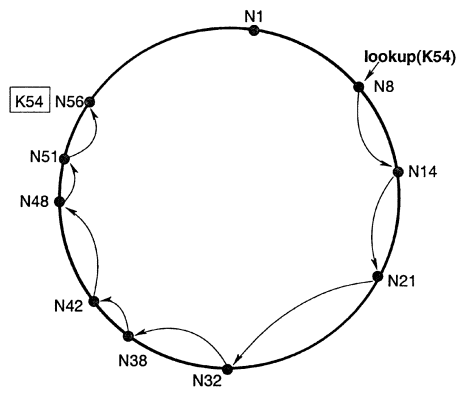
\includegraphics[width=5cm]{img/chord-lookup.png} }}%
\qquad
\subfloat[Can file query mechanism \cite{p2p-survey-1}]{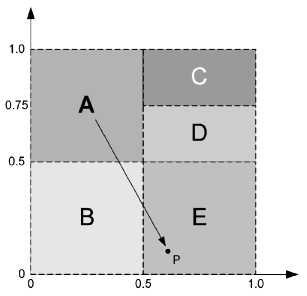
\includegraphics[width=5cm]{img/can-lookup.png} }%
\caption{Examples of structured P2P query mechanisms that utilize DHTs}
\label{fig:dht-usage}
\end{figure}

\subsection{Effects to the Network Infrastructure}

    Historically, ISPs have deemed P2P traffic as unideal or even undesirable.
    Besides the aforementioned illegality precedent that is tied to P2P applications, the overall properties of P2P networks make them unappealing to support - due to the distributed nature of these types of networks, the overall traffic is less predictable, with the higher upload traffic volume in edge networks requiring infrastructural investments, and the network-agnostic operation mode of P2P applications leads to inefficient and uncooperative network resource usage.

    P2P networks who neither have structure nor a central point of control have to utilize content retrieval methods which are bound to be less efficient than their counterparts.
    However, architectures which fit in these categories mostly do so with a clear purpose - Gnutella's decentralized nature makes it very hard for individual nodes or external entities to regulate what can happen in the network (such as enforce legal actions), and its lack of structure simplifies the architecture and reduces the overall effort to bootstrap to the overlay, making it a good fit for applications with a high peer churn rate.
    Similarly, FreeHaven, an also unstructured and decentralized P2P protocol, has architectural decisions fit a very specific use case, as it "emphasizes distributed, reliable, and anonymous storage over efficient retrieval" \cite{freehaven}.
    The lack of systematic means to efficiently locate content by these P2P architectures means that more ad-hoc methods have to be used, which are less efficient and thus incur in bigger workloads for ISPs - the usage of query flooding by Gnutella and message broadcasting by FreeHaven are examples of this.

    The usage of structure by P2P networks can, as stated before, result in more efficient content and peer location algorithms.
    However, maintaining such structure also requires a chunk of ISP resources, as peers need to periodically update others, as well as react to peers entering and leaving the overlay.
    The usage of key-value mappings with DHTs can also have potential to be ISP unfriendly as the hash function's purpose is to evenly distribute resources over the network - whilst such property is certainly advantageous in certain use cases, doing so removes any  applicational context that exists in the content - for example, grouping resources which belong to the same web page can't be done, as they will be individually hashed and spread out.

    A first point of improvement is optimizations made in the applications themselves to less degrade network resources.
    An example of these can be visualized in Figure \ref{fig:p2p-optimization}.
    To the left, a point of optimization in the Chord system would try to reduce the number of query messages per resource by increasing the number of successors a given node knows.
    That way, the querying node can instead query not for the single successor it knows, but instead by querying for the one who's ID immediately precedes the content's, thus insuring a least number of hops to retrieve the message.
    This thus reduces the total amount of traffic on the network and improves application times.
    To the right, a point of optimization in the Gnutella system could try to tackle the usage of query flooding to locate data, as such flooding grows exponentially and thus intakes a massive toll on network resources.
    A query flooding system would not be as prejudicial if content was equally scattered throughout the overlay and a given content was an amount of hops away which was average to the overlay's diameter.
    However, as concluded by extensive analysis of user traffic on Gnutella, nearly 70\% of users share no files and nearly 50\% of all responses are returned by the top 1\% of sharing hosts \cite{freeriding-gnutella}.
    An attempt to improve this situation was done in \cite{altruistic-gnutella}, which injected a special node that interfaced with the Gnutella protocol and acted as a cache and load balancer.
    Much like the previous example, these optimizations have the benefit of reduced network resource usage and increased application performance.

\begin{figure}%
\centering
\subfloat[Chord file query mechamism with larger neighbour knowledge\cite{stoica2003}]{{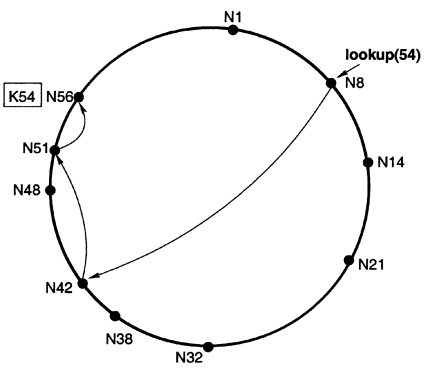
\includegraphics[width=6cm]{img/chord-lookup-efficient.png}}}%
\qquad
\subfloat[Gnutella file query mechanism with prior caching]{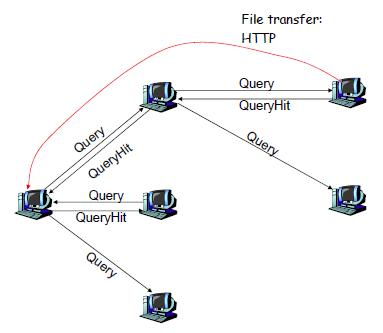
\includegraphics[width=6cm]{img/gnutella-flood-efficient.png} }%
\caption{Examples of P2P query mechanisms optimized from their counterparts}
\label{fig:p2p-optimization}
\end{figure}

    Regardless of the many ways through which P2P systems can operate, e.g., in regards to structural mechanisms and centralization, and even disregarding potential application optimizations, no classic P2P system operates in full understanding of the underlying network topology, nor with cooperative behavior with ISPs.
    The network-agnostic manner under which they operate results in overlay networks which are layered on top of the underlay where they run, as exemplified in Figure \ref{fig:overlay-underlay} - as P2P applications are network-agnostic, two neighboring peers could exist in completely different contexts on the common network layer - for example, they could either be connected by a single data link or be multiple network provider domains away from each other.

\begin{figure}[!h]
\centering
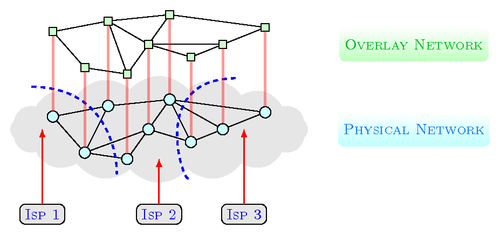
\includegraphics[scale=3.0]{img/p2p-topology.png}
\caption{Example demonstration of an overlay network and corresponding physical layer.}
\label{fig:overlay-underlay}
\end{figure}

    P2P application's inability to localize traffic is seen as a big problem - as concluded by \cite{liao2014}, ISPs face bottleneck bandwidth pressure in the large scale Internet of the future, in particular from P2P applications, and an increase in P2P users is not necessarily harmful, and perhaps helpful, if traffic locality can be boosted.
    Thus, there is a necessity to ensuring that peers prefer to generate traffic within network locality over traffic which crosses network borders.
    A first step would be increasing the availability of content within network boundaries, through means such as cache injections or peer content serving incentives.
    Given that content resides locally, a second step would be that P2P applications have a network-aware vision of the overlay, which does not happen with classic P2P protocols.
    This issue is particularly damaging in P2P applications whenever neighbours are selected, and whenever a service exists redundantly in the network and a decision must be made in regards to what peer or collection of peers to consume the service from.
    If it indeed is the case that P2P applications are not locality aware, it can easily be seen how this can be an issue: for P2P applications, choosing peers which are not local to the querying peer may result in more time to retrieve the requested contents; for ISPs, bad network resources management can incur in higher operational costs, and may degrade overall network performance in many cases, e.g., by not being able to stop applications from overusing inter-AS links which usually are network bottlenecks (a conventional wisdom demonstrated in \cite{akella}) and which, due to peering agreements with other ISPs, are less desirable to be overused due to peering costs.
    If the P2P application were to attempt to choose the peers that would most effectively serve the querying peer, it could depend on privileged information that the ISP has on the network's properties and current status (such as the inherent network topology, link properties, or scheduled server maintenance).
    Attempting to optimize peer selection without a co-operational channel with ISPs would be sub-optimal as not enough information is known, and could perhaps even be more damaging with the wrong techniques - consider a peer selection algorithm that chooses the peers with lowest RTT of a probing ping message, whilst having no indication on available end-to-end bandwidth.
    Likewise, attributing neighborship via geographical proximity - much like the CAN architecture does - whilst initially seems like a good step in location awareness, may also not be optimal - ISPs may not always prefer geographical proximity in connections, as peers could be very geographically close but residing in different ASs and thus separated by costly links.
    Other peer-selection techniques focus on randomly selecting nodes, which is simple and resilient to peer churn \cite{qin2009}, but as a consequence is sub-optimal on network resource usage as no network consideration exists.
    It is fair to say that no P2P application can act with full ISP consideration without directly cooperating with it, and simple heuristics should be, whenever possible, traded for methods where full cooperation with the underlay is done - that is, if the needs of both layers are being considered.

    Indeed, it is the case that current P2P solutions are ISP-unfriendly.
    More concretely, \cite{isp-p2p-tussle} shares the view that P2P applications and ISPs are in a tussle since P2P applications generate traffic which favours the application's needs whilst ignoring the ISP's, which in turn upsets the ISP's business model.
    To name a few examples, BitTorrent seems to employ peer selection algorithms which do not consider the underlay network, which can result in degraded download performance and increased load on ISPs \cite{qin2009}.
    \cite{karagiannis} found that since this protocol is locality unaware, 70-90\% of existing local content was found to be downloaded from external peers and suggests that locality-aware content distribution algorithms could significantly reduce the total amount of traffic generated.
    Likewise, Gnutella generates traffic which is not ideal, as it may have to cross ISP network boundaries multiple times \cite{estimating-gnutella} due to the same fundamental issue stated before - an application layer that operates in disregard to the network underlay it runs on.

    As \cite{dan-Commag10} describes, the ongoing friction between the overlay and underlay layers has made it to the point where ISPs have chosen to throttle the bandwidth of P2P traffic, or even outright blocking it.
    In return, P2P applications have tried to mask their presence to bypass such restrictions via tunnelling or using non-standard and random port numbers.
    This is an unsustainable system that is bound to hurt both ISP profit and application functionality, and a strategy of cooperation between the overlay and underlay layers is crucial to guarantee that the requirements of both parties are met.


\section{Content Distribution Networks (CDNs)}

\subsection{Concepts and applications}

    A content distribution network (CDN), as the name implies, is a network specifically designed with its main focus on distributing content to a set of end users.
    Its design allows for the alleviation of performance bottlenecks on the Internet generated by client requests, and has been recently been considered a powerful tool as a response to the existing high demand for media content, which has a huge share of the global Internet traffic of today.

    Functionalities of CDNs include \cite{cdn-survey}:

    \begin{itemize}
        \item \textbf{Content outsourcing and distribution:} Replicate content throughout the network into edge servers, which are deployed nearby end users.
            Doing so allows CDN clients to pay for their content to be hosted on these edge servers, and in doing so guaranteeing that their content is quickly accessible by end users.
        \item \textbf{Request redirection:} Direct a content request to the most appropriate edge server at a given time.
            This redirection is done considering relevant network properties, such as geographical locations and current server loads.
        \item \textbf{Content negotiation} Leverage the network's properties to fit the needs of its clients through negotiation.
        \item \textbf{Management:} Manage the distribution network, which includes accounting, monitoring, statistical analysis on content consumption, etc.
            A close management of the distribution network is important for its business model, as, besides being needed for a billing system, allows for a better understanding for the usage patterns of the network, which is helpful information in better engineering the network to most optimally serve content with increased revenue and decreased costs.
    \end{itemize}

    The current focus of CDNs is thus to provide content, e.g., web pages, documents, photos, videos, or media-related streams, with high availability and performance.
    The strategy used by CDNs to guarantee a satisfying quality of experience (QoE) on a global scale is the deployment of content close to the end-user - a CDN contains many nodes which are geographically spread throughout the globe and close to the users they wish to serve, and whenever such users request for content, they are routed to the node which is closest to them (\cite{cookbook}).
    Data replication to servers which are strategically placed closest to end-users, coupled with good means to properly redirect such users to the most attractive edge server, is what allows content to be available more often and more quickly.
    These are undoubtedly attractive features in the world of e-commerce, where user QoE can dictate much of the profit - for example, Akamai, one of the leaders in CDN-related services, ran a research concluding, among other things (\cite{akamai}):

\begin{itemize}
    \item A 100 millisecond slower webpage loading speed can result with a 7\% drop in sales
    \item A 2 seconds slower webpage loading speed can almost double the number of visitors who end up abandoning their carts
    \item 53\% of users who use smartphones to visit web stores won’t make the sale if the webpage takes more than 3 seconds to fully load
    \item 28\% of users won’t return to the same web store if they think it takes too long to load
    \item A 250 millisecond faster loading time proved to keep users from visiting a competitor web store
\end{itemize}{}

    It should then come to no surprise that streaming services such as Netflix and Youtube, who now reach a global scale and whose utility is highly dependant on their high availability and low transmission delay, routinely use CDN solutions.
    More broadly, typical CDN customers include media and Internet advertisement companies, data centers, ISPs, online music retailers, mobile operators, etc \cite{cdn-survey}.
    Indeed, companies that wish to provide a given service in the web and who wish to have global presence routinely partner with companies whose focus is providing content delivery services, with popular examples being Akamai, CloudFlare, or Amazon Cloudfront.
    Coupled with the promise of highly available and quick content retrieval, these companies also couple other attractive services, such as firewalls and DDoS protection.
    The Internet's currently most targeted use for media consumption has made it so CDNs and their providers have an important role in dictating a very considerable percentage of flow of traffic in ISP-owned infrastructures, and as such their study and improvement is quite important, as are the efforts to increase harmonious behaviours between content delivery applications and service providers, with the goal in mind being network resource efficiency to guarantee that ISPs can remain operational and applications can provide a satisfiable user experience.

\subsection{Architecture}

    Figure \ref{fig:cdn-conceptual-architecture} represents a high-level conceptual architecture of a CDN.
    The true power of a CDN comes from its strategically deployed cluster of replicated server - at a global scale, this implies having those servers geographically dispersed and located in or nearby networks with large content demand.
    The origin server possesses the content that is to be served, and the bootstrapping process has it uploaded into the network, which is afterwards replicated.

\begin{figure}[!h]
\centering
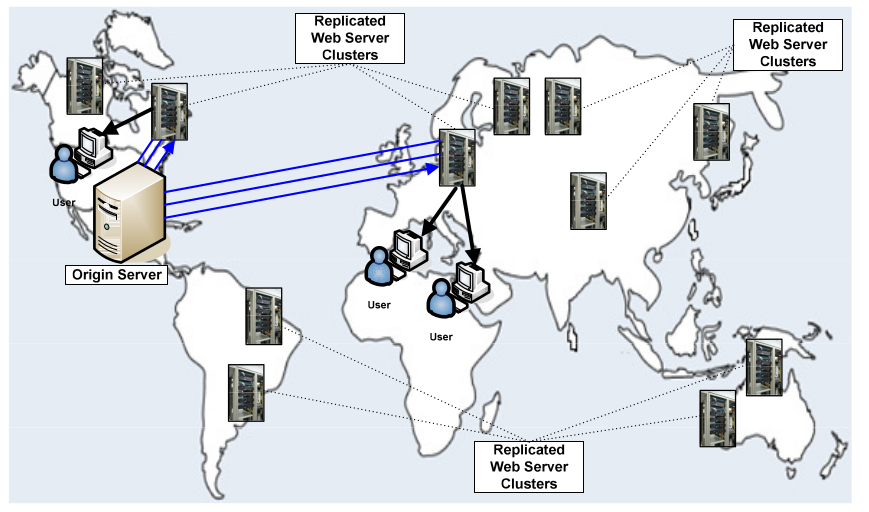
\includegraphics[scale=0.5]{img/cdn-architecture.png}
\caption{Conceptual architecture of a CDN \cite{cdn-survey}}
\label{fig:cdn-conceptual-architecture}
\end{figure}

    Figure \ref{fig:cdn-request-routing} displays how, conceptually, the request routing functionality of CDNs.
    As can be seen, the request is firstly directed to the origin server, and serves only light, basic content.
    In the situation where heavy static content is requested, the origin server redirects the request to the CDN provider, which utilizes a selection algorithm select the most appropriate edge server to serve the content to the end user.

\begin{figure}[ht]
\centering
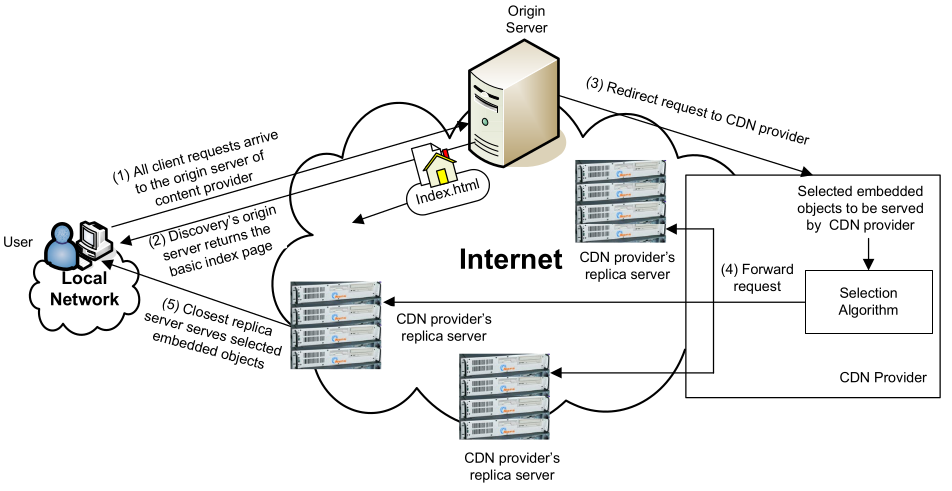
\includegraphics[scale=0.5]{img/cdn-request-routing.png}
\caption{Request routing functionality of a CDN \cite{cdn-survey}}
\label{fig:cdn-request-routing}
\end{figure}

    The Request routing mechanism is the one that informs a given user to a given edge server.
    The prevalent approaches are, according to \cite{wichtlhuber2017}, the following:

\begin{itemize}
    \item \textbf{DNS request routing}: The user must first resolve a domain name to retrieve a content. The CDN's DNS processes such request and, utilizing the user's IP address, historical measurement information and current server loads, responds with the edge server that seems most fitting to provide such content.
    \item \textbf{HTTP request routing}: Content is firstly requested to a nearby proxy server, which in turn answers with an HTTP redirect to be resolved by the client in order to find the content.
        The HTTP requests can occur in subsequent rounds and can also use DNS knowledge when the redirection domain must be resolved.
    \item \textbf{Anycast request routing}: The CDN provider announces an anycast prefix to the network.
        Whenever a router receives multiple announcements to the same prefix incoming from different locations, it chooses one considering some custom criteria, usually being AS hop count and Interior Gateway Protocol (IGP) weight.
        Thus, different routers can have a given anycast address mapped to different hosts, meaning the ones that are most suitable for that particular router.
\end{itemize}{}

    These mechanisms are also discussed in \cite{cdn-survey}, but also add:

\begin{itemize}
    \item \textbf{Global server load balancing (GSLB):} Service nodes, consisting in edge servers and GSLB-enabled web switches are interconnected in a network.
        Individual nodes possess global awareness of the network, meaning the status of each individual server.
        With edge servers having more information on the health and status of all other candidate edge servers, and the web switches acting as authoritative DNS servers, the network can enables the support of a global-wide server load balancing mechanism that intakes dynamic server information.
    \item \textbf{URL rewriting:} The origin server redirects the end user via dynamically altering the host pages' URL links.
    \item \textbf{CDN peering:} An extension of a single CDN network to multiple, connected CDNs which serve content on behalf of others when appropriate.
        This is helpful to extend the domain reachability of a single CDN, increase fault tolerance, and ability achieve better performance with more candidate servers to choose and balance loads from.
\end{itemize}

    It is vital that a CDN possesses a clear view of the network performance inside its domain.
    \cite{cdn-survey} lists important metrics which are used to measure CDN performance:

    \begin{itemize}
        \item Geographical proximity of end users
        \item Path latency
        \item Path packet loss
        \item Path Bandwidth
        \item Path startup time
        \item Path frame rate
        \item Server load
    \end{itemize}

    Means through which these metrics are retrieved by the network include network probing of relevant entities (in particular the end users), traffic monitoring of end user to surrogate server communications, and surrogate server feedback retrieval via application requests or measurement probings \cite{cdn-survey} \cite{akamai-report}.

    Having a clear understanding of CDN performance is important for system management in two fronts - firstly, through performance evaluation, by providing the billing and monitoring modules the verification of how the network is faring at its task of caching and delivering content on behalf of clients; secondly, through performance optimization, by providing the logical layer an updated view on network status, serving as contextual input that the system uses to better reason on how to act - for example, in regards to the caching and request routing mechanisms.

\subsection{Effects to the Network Infrastructure}

    As previously discussed, CDNs came as a tool to strategically position content on the network in such a way that it can more quickly and more reliably be retrieved by an end-user.
    These CDN systems are then inherently a means of optimizing network resource utilization in the application layer, and thus are of great interest for ISPs as their mode of operation, if done properly, can be very appealing not only to them but also to end-users that use applications leveraging these networks.

    The usage of a single content-providing server (or a limited set of them) which is far away from the content supply that in turn can have a large geographical distribution is prone to overloading such server and path congestion if a big enough scale is achieved.
    The usage of data caches is a classic solution for network inefficiency problems, which is used by CDNs as a means to replicate content to strategic locations to better serve users, with the added benefit for ISPs that their network resources are efficiently used, with the ability of reducing the total amount of used bandwidth needed for a service to operate - as data travels a shortened total amount of network hops from data source to points of data demand - and reducing congestion of inter-domain links - as data caches will reside locally and redistribute traffic away from highly shared network links.
    It can thus be stated that the relationship between CDNs and ISPs is a win-win situation because efficient network usage has consequentially better service quality.

    However, there does not seem to exist proper cohesion with the underlying network infrastructure by CDNs during application operations.
    As stated by Akamai, a leader in Content Delivery Network services, in their report \cite{akamai-report}, the large scale and complexity of the Internet, where it takes well over 650 networks to reach 90\% of all access traffic, adds to it many challenges to the CDN's role of content delivery - in particular, whilst good investment seems to exist at the first and last mile of internet access (website hosting and end users, respectively), there seems to be little economic incentive to invest in the middle mile, composed of peering points shared among networks, which in turn become network bottlenecks and become susceptible to cause increased traffic packet loss and latency, making inter-network communications unreliable - and loose coordination between autonomous networks with internal biases is pointed as a main cause.
    Due to this, even a well provisioned data center will be at the mercy of the various inter-network bottlenecks that may arrive, and performance takes a hit.
    In fact, the paper suggests a clean-slate redesign of the Internet as a potential solution to its many problems - besides the peering point congestion mentioned above, inefficient routing protocols, unreliable networks, inefficient communications protocols, and application limitations also add to the problematic - but such a redesign to a massive and highly invested global infrastructure doesn't seem plausible.

    In alternative to proper network infrastructural insight, CDNs have to rely on network probing, traffic monitoring, and server feedback, as seen above.
    Even assuming that these are sufficient, the usage of probing techniques will incur in overhead traffic on the network, and even worse if other overlay networks do so as well, in a redundant fashion.
    Similarly, traffic monitoring to extract end-to-end path metrics to end users requires resources and takes time, and may also incur in redundant operations if other overlay networks are utilizing the same strategy.
    Regarding this topic, projects such as IDMaps \cite{IDMaps} and GNP \cite{GNP} described architectures for a global distance estimation service, leveraging measurements made by specialized nodes that retrieve raw network data, and heuristics provide scalable and functionally reliable path costs in metrics such as bandwidth and latency.
    These then consist on systems that centralize and share network probing results into querying entities, thus minimizing overhead traffic on the network, especially between popular Internet points.
    Such advantage goes outside of the CDN realm, being thus useful for any overlay-residing application that wants to utilize network probing to be more underway-aware.

    Advantageous as network probing and traffic monitoring mechanisms can be for CDNs to proper conduct request routing and caching decisions, a case must me made against proper application-infrastructure synergy during decision making in the overlay.
    Much like P2P systems, to infer on network status by measuring it - versus receiving input by trustworthy, authoritative, entities that possess privileged network information, such as ISP administrators - is insufficient.
    Attributing edge servers to end-users entirely on geographical data was previously discussed as being a non-optimal way of assessing node selection at the application layer.
    Whilst it may be intuitive that the best edge server to serve an end-user would be the one most geographically close to it, that is not always necessarily the case, much like was discussed in similar strategies used in P2P systems.
    Again, much like in the scenario of peer selection in P2P systems, the usage of network measurements made by the CDN itself to better pick the appropriate end-server, while it could potentially be beneficial, it could certainly be improved if it used additional, hard to retrieve data that only ISPs or other privileged entities could possess, and which are at a position to guide applications in the infrastructure with whom they have detailed knowledge.
    There indeed seems to be a consequential coupling between overlay decisions in the CDN systems and the underlying infrastructure - do the CDNs not take ISP input when redirecting clients, suboptimal choices can be made that would be prone for bottleneck congestion, and would ISPs take all the responsibility in redirection, user-level application QoS agreements might not be met.
        \cite{pushing-cdn-isp-collaboration} states that this lack of awareness to network status is indeed problematic for CDN systems, listing end-user mismatching to edge servers based on dubious DNS-based location binning and resource consuming, non exact methods to detect bottlenecks, as well as lack of agility in server deployment in ideal locations.
        This is a view shared by \cite{cdn-isp-cooperations}, which adds that these problems reside in a share medium that raises the opportunity for cooperative behavior that would enable better application performance and optimized ISP resource utilization.
        In fact, Akamai themselves have formed content delivery strategic alliances with major ISPs, such as AT\&T, Orange, Swisscom and KT \cite{pushing-cdn-isp-collaboration}, which hints at this type of partnership being the norm for content distribution technologies.

        ISP input permits applications to act in a more network-aware fashion than without it - whereas pairing overlay nodes or deploying edge servers in terms of geographic distance, RTT distance, or any other metric, may give further decision power than a purely network-agnostic overlay system, proper guidance by ISPs could help pairing based on more complex metrics that, besides the aforementioned ones, also consider ISP objectives - for example, to minimize network distance, avoid bottlenecks, locate content caches, etc.
        This is further heightened if many other overlays coordinate their efforts with the ISP, which can now in turn orchestrate its traffic, which would previously be generated with no input from it, in such a way that maximizes network resource utilization and, consequently, application performance - this is an important point to consider because one-sided application decisions cannot fully grasp network status nor can they coordinate efforts with other applications for a more harmonious, and thus efficient, Internet.


    \section{Server mirroring}

    \textbf{[Change the section 'server mirroring' and talk about the classic server-client architecture instead, and in it bring up the server mirroring technique.]}
    \todo{finish this}

    \subsection{Concepts and applications}

        Server mirroring is the act of continuously replicating a server into another, essentially creating an exact copy of it that is now accessible as if it were the original.
        Whilst CDNs aim at replicating chunks of contents wherever it may be necessary, the act of server mirroring performs an integral copy of a server which is self sufficient at serving a given client, as long as it periodically checks up with the primary server for synchronization \todo{cite}.
        It is a standard business strategy that uses redundancy as a means to increase reliability, availability and performance.
        The existence of many servers that perform the same task means that these can be strategically chosen to serve a client in a given situation, e.g., by selecting the one that has small end-to-end message delay and little current server load.
        Figure \ref{fig:mint-mirrors} shows an application of this, where multiple server mirrors exist to deliver software packages to the Linux Mint distribution. The user has the choice to manually select one of these mirrors, and ideally chooses the one that is most fitting to them.

    \begin{figure}[!h]
    \centering
    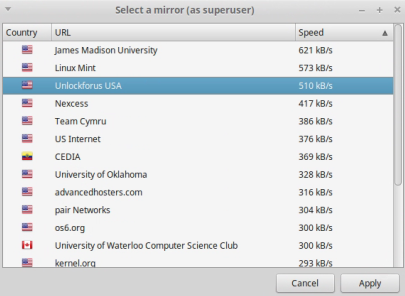
\includegraphics[scale=1.0]{mint-mirror.png}
    \caption{Linux Mint prompt to select a software repository mirror}
    \label{fig:mint-mirrors}
    \end{figure}

    \subsection{Effects to network infrastructure}

        Much like the content replication utilized in CDNs, an integral replication of a main server proves itself as an advantageous tool capable of delivering services more closely to users, and as such allows the reduction of total amount of bandwidth used to serve all clients.
        Much like all previous use cases discussed before, optimizing application traffic is crucial to guarantee good network resource usage, and in case of server mirroring it comes down to good strategical deployment and dynamic, intelligent algorithms to properly attribute mirrors to requesting end-users.
        Giving end-users the choice to manually select the serving mirror seems problematic, as application-generated traffic is not optimized.
        In fact, considering the Linux Mint software package distribution discussed above, despite currently existing seventy mirrors deployed throughout the globe to fit this role, a large number of these remains mostly unused whilst the main and default server is constantly prone to overworking \cite{mint-article}.
        It can be stated that end-users both don't care enough to optimize traffic nor do they have enough information to properly do so even if they did.
        Deployment of server mirrors is a great tool that brings with it the issue of optimizing server selection, and much like all examples given so far, traffic generated by applications can be firstly optimized by the applications themselves if they consider static and dynamic information of the network they operate on.


    \section{Traffic optimization by applications and layer-cooperative approaches}

        This section serves to display the proposed solutions and existing implementations that have been made in the attempt to optimize application traffic utilizing network information.
        Given the increasing scale of the Internet as a near ubiquitous system, and increasing tension between service providers and applications, it comes as no surprise that the area of layer cooperation has been through exhaustive work.
        Many solutions have been devised for specific use cases, with varying degrees of power to each one of the layers.

        \subsection{Peer-to-peer applications}

        Many different mechanisms have been developed with the goal of decreasing tensions between ISPs and P2P applications, which is a subset of the general layer cooperation problem.
        Figure \ref{fig:p2p-isp-interactions} represents a grouping proposed by \cite{dan-Commag10} where such mechanisms are ordered in agreement with how much involvement the P2P systems and ISPs have. These classes are as follows:

    \begin{itemize}
        \item \textbf{Class 1}:
            There is not much interference in the overlay by ISPs nor are P2P systems cooperative.
            Instead, ISPs apply traffic engineering methods to selectively favour types of traffic.
            This is usually done to guarantee certain QoS levels to some classes of traffic, which are then to be treated favourably at the forwarding and routing levels.
            Examples of such techniques are DiffServ, Multi-Topology Routing (MTR) and MultiProtocol Label Switching (MPLS).
            These classes of methods do not fix the underlying application behaviour, but are instead used to control preexisting traffic.
            As such, the peers' routing decisions are not affected and P2P traffic still remains non localized.
        \item \textbf{Class 2}:
            There is ISP intervention in the overlay in such a way that peers continue normal operation without realizing that such interventions occur.
            This can be reached via the use of proxies that can affect the control plane with the redirection of content requests to local peers, or at the data plane with content caches which act as normal peers and are strategically placed in the network.
            These methods are advantageous because they do not require any changes to P2P protocols, because the ISP has an active role in molding to the overlay, intercept traffic, and either help or guide it in a way that favours them.
            Indeed, these techniques can be proven to work , as concluded in \cite{dan-Commag10}, and put into practice, for example, in \cite{programmable-trackers} and \cite{configurable-trackers} via the specification of a BitTorrent tracker that is programmable to allow for P2P qualitative differentiation and ISP-cooperative traffic engineering that could help reduce inter-domain traffic significantly.
            Additionally, in \cite{freeriding-gnutella} with the injection of special nodes on the Gnutella overlay which interface with the base protocol nodes but with the added caching and load-balancing mechanisms.
            This seemed necessary after concluding with extensive analysis of user traffic that nearly 70\% of users share no files and nearly 50\% of all responses are returned by the top 1\% of sharing hosts \cite{freeriding-gnutella}, and such a solution  helps minimize the total size of query floods and more evenly distribute content on the network for decreased network resources usage.
            However, this class of mechanisms are not without their challenges - firstly, it involves much effort by ISPs, as it requires structural upgrades and constant adaptiveness to new and changing P2P protocols.
            Perhaps worse, even considering proper budget and maintenance, such methods can prove themselves to be not possible at all - for legal reasons, as data caches could possibly contain illegal content; and for technical reasons, since the packet inspection required by ISPs to detect and steer P2P traffic may be blocked due to the peer's attempts to mask its traffic.
        \item \textbf{Class 3}:
            Relative to previous classes, the active role is switched and it is the P2P system itself that acts in regards to the underlay it operates on, but without ISP involvement.
            Peers probe the neighboring network elements as a way to get more familiar to connection properties, and act on these probings during operation, e.g., when choosing neighbours to construct the overlay network with, or when choosing to whom request a given resource.
            Whilst these methods can be advantageous for both applications and ISPs, it can't be assumed that to always be the case - as peers have no ISP input, they cannot have a full scope on the network and ISP needs, and as such these application optimizations can end up being more hurtful than helpful.
            For example, consider a scenario where a peer uses RTT measurements to choose between two candidate peers, but the one that is geographically closest to it belongs to another AS, and his preferring it for content supply would incur in more costs.
            The paper describes this class as a "win-not-lose" situation, meaning that while the P2P system can, in the right circumstances, improve their performance via measurement-oriented strategies, the ability to act beneficially to the underlay without any feedback from ISPs cannot be guaranteed.
            Such an example of class 3 mechanisms could be seen in \cite{qin2009}, which improved BitTorrent's download performance and even managed to reduce ISPs' backbone and cross-ISP traffic.
            The technique consisted in having peers send traceroute measurements to the tracker, which in turn grouped them into local, intra-ISP and inter-ISP groups, with the assumption that inter-ISP links generally have much more latency than the rest.
            As peers would later query the tracker for content, the returned peer list would be biased in such a way that promotes traffic locality.
            Another example of this is \cite{kim2011}, which devised a CDN-P2P hybrid where peers utilize RTT measurements to group themselves by separate orders of geographical proximity with the same intent of the previous example, which is to localize traffic whenever possible.
            This technique also proved itself to be advantageous, as the solution was more efficient in terms of total service disruption time when compared to a previous iteration of the hybrid architecture which used random peer selection to look up available target peers.
            As a final example, \cite{topology-aware-p2p-server-selection} proposed a node binning scheme that groups nodes of similar orders of magnitude of RTT values to pre-defined landmarks, and utilized such scheme for topology-aware overlay construction mechanisms in some unstructured and structured P2P overlays.
            Results allowed to conclude that even surface levels of relative topological distance were advantageous and can significantly improve application performance.

        \item \textbf{Class 4}:
            Full and active cooperation exists between the ISPs and P2P systems.
            The role of the ISPs is to provide information and guidance, and P2P systems let themselves be influenced during operation.
            It is the methodology that most comes close to a mutually advantageous scenario for both parties, given that they both keep the entire group's needs in mind.
            For example, \cite{locality-aware-p2p} proposes an oracle that receives as input from a querying peer a list of candidate peers, and ranks them in order of proximity to that peer; such method was tested in simulation and proven to decrease negotiation traffic and improve scalability of P2P networks.
            Similarly, \cite{configurable-trackers} proposes a framework for programmable trackers in a BitTorrent trackers scenario, providing an interface to directly define tracker behavior which, given ISP input, can provide a collaborative scenario between ISPs and the BitTorrent users in an attempt to, among other things, localize traffic.
            The functional intent is that the oracle possesses privileged network information and acts on it to provide guidance to querying applications, and thus has the liberty to impose policies and optimizations, e.g., pair peers which are the least number of network hops apart via a Dijkstra algorithm.
            Another more complex approach that could be used by the oracle proposed by \cite{han2009}, which contains algorithms to dictate peer selection, task assignment and rate allocation.
            The method requires the full network topology as input - including link capacities and peer service costs - to minimize file downloading time and cost.
            The oracle would also be free to enforce ISP biases as its preferences by modifying such algorithms as to, for example, minimize usage of costly links (such as inter-AS ones).
            The ALTO working group - whose work this thesis attempts to materialize into a working system and further extend its features - was formed to standardize the oracle-user scenario so it could be properly used in many situations at the scale of the Internet.

    \end{itemize}

    \begin{figure}[!h]
    \centering
    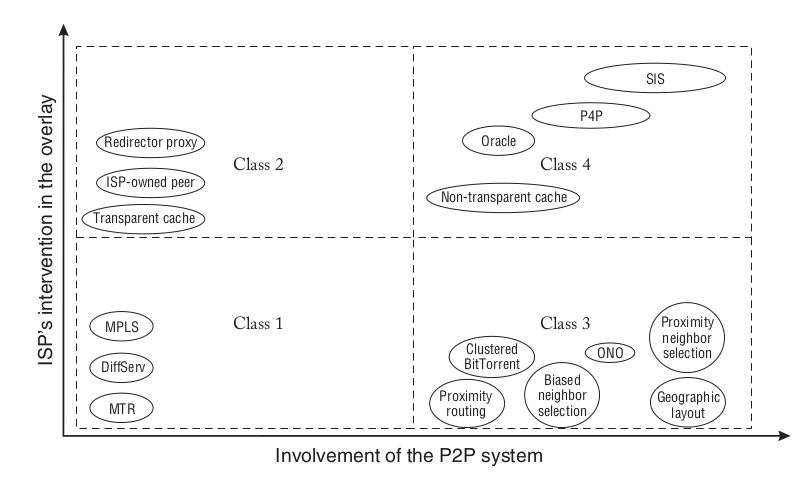
\includegraphics[scale=0.65]{img/approaches-isp-p2p.png}
    \caption{Existing approaches to decrease tension between P2P applications and ISPs (\cite{dan-Commag10})}
    \label{fig:p2p-isp-interactions}
    \end{figure}

    \subsection{Content Distribution Networks}

        Given the current share that CDNs have on global Internet traffic of today, coupled with the demand for a good QoE by end-users, it should come to no surprise that this application domain has also been through efforts to optimize its traffic.
        One such way to do so is to optimize client query redirection, i.e., better choose which edge server should be attributed to an end-user when a name resolution is requested for some content.

        \cite{gromov2014} considers a CDN built to deliver video data where some given set of content exists redundantly in many edge-servers, and argues for an algorithm where the choice is made to optimize client download time, which in turn has to consider the network parameters at time of request, as well as current server load.

        Some simple, flexible and scalable techniques exist that utilize no ISP input.
        For example, \cite{topology-aware-p2p-server-selection}, mentioned previously for its P2P overlay construction with a binning technique based on RTT to landmarks, also utilized such binning technique for improved server selection.
        Similarly, IETF tackled application traffic optimization via multi-CDN cooperation, and devised a problem statement in regards to Content Distribution Network Interconnection (CDNI) \cite{cdni-problem-statement}, which outlines the efforts needed to specify a set of interfaces that allow for the interconnections of many CDNs, with the added benefits that a multi-CDN system, over an individualistic one, will have better properties, i.e., availability, coverage, and capabilities, as well as better QoE for the end user, and reduced delivery costs.
        The four devised interfaces (CDNI Control interface, CDNI Request Routing interface, CDNI Metadata interface, and CDNI Logging interface) are all control plane interfaces to be operated at the application layer, and the group states that no new application protocol needs to be devised, and instead existing ones could be leveraged, e.g., HTTP, Atom publishing protocol, XMPP, and in particular to the CDNI Request Routing interface, the ALTO protocol who's the focus of this work.

        \cite{cdn-isp-cooperations} argues for the advantage of cdn-isp cooperative interactions and overviews three relevant strategies that will be now discussed briefly: Provider-aided Distance Information System (PaDIS) \cite{pfa-10} is a system deployed and controlled by ISPs that monitors the network by listening to EGP and IGP messages and contains a privileged view of the topology and its status, and provides a service that ranks host-client pairs in regards to, for example, delay, bandwidth, or hop count, and experimental testings concluded that download times of content provided by CDNs that utilize PaDIS can be improved to a factor of four and gives much flexibility for ISPs for traffic engineering; Content-aware Traffic Engineering (CaTE) \cite{fps-12} is designed in a similar manner to PaDIS but requires no client-side configuration, and experimental results concluded in network wide traffic reduction by 15\%, decrease in ISP link utilization by 40\% and increased user-server performance; Network Platform as a Service (NetPaaS) \cite{fpl-13} was devised to fulfill two key enablers in a fruitful CDN-ISP collaboration - user-server assignment, as it was tackled in the previous two examples, and server allocation, i.e. where should a CDN deploy its servers and its contents, thus having increased functionality over the previous two examples, and concluding that, beyond the common advantages of increased application performance and better ISP traffic control over network resource utilizations, this system facilitates the task of server allocation for CDNs, reinforcing the discussed advantages and simplifying the task for CDNs.
        Still in the topic of CDN's edge server selection, \cite{wichtlhuber2017} suggests a way of optimizing anycast request routing, which differs from the DNS-oriented request routing techniques, which, while very light in terms of network engineering and infrastructural overhead when compared to existing alternatives whilst maintaining a close to optimum network path, it sacrifices flexibility to do so, as it is agnostic to the network's status and not much network engineering can thus be done.
        As such, the work proposes anycast request routing utilizing software defined networking (SDN), where load balancing is made at the ISP network with help of CDN-provided additional information.
        This example of layer cooperation can allow for many optimization opportunities that leverage an existing and low-maintenance mean of request routing with the flexibility achieved with SDN solutions.

        \subsection{Server-client applications}

        Attempting to optimize web server selection, \cite{kenichi} argues that DNS-oriented solutions, which select the nearest server but also employing load balancing, may not be the best at optimizing server-client QoS levels.
        Instead, it is proposed that selection is based on QoS measurements, from which three types are distinguished: a static method, such as choice based on least number of hops to server (which is unlikely to change); a dynamic method, consisting on dynamic instantaneous probing of the network to monitor, for example, round-trip time (RTT) delay to the servers; and statistical methods, which decide based on a larger set of measurements made in various points in time.
        Utilizing the latter method, RTT measurements and web-related request benchmarking is made, such as time to establish TCP connection, elapsed time from GET HTTP method to first packet received, time to retrieve data fully, etc, every five minutes and spanning several weeks.
        The work concluded that statistical methods used to select between multiple equal web servers had high correlation with download time from the selected server, but optimizations should be evaluated in regards to computer workload and the amount of probing traffic.
        Tackling a similar challenge, \cite{swain} proposes a method of server mirror selection which is better optimized than the more popular approach of giving the user the selecting choice.
        The proposed solution's architecture consists of two types of agents: a client agent, which monitors the mirror server it was deployed in and stores static information, e.g., geographical location of server and maximum capacity, and dynamic information, e.g., current load and bandwidth.
        This information is then sent to the other role of the architecture, the server agent, which compiles it and acts as an oracle that is queried by users whenever mirror selection is needed, replying with a ranking of candidate servers based on bayesian networks.

        Congruent to the task of optimizing network traffic with layer cooperation, \cite{adaptable-overlay} proposes a reconfigurable and adaptable overlay multicast system, further optimizing the multicast strategy - used for group communication as a means to reduce redundant traffic - and leveraging collaborative efforts between it and the ISPs to construct multicast distribution trees whilst integrating traffic engineering mechanisms for the task of network usage optimization.

        \subsection{Edge Computing}

        \textbf{[ALTO has a solution for server footprinting and connectivity that gives users more information about the cloud, and thus lets them better decide how to better rent servers for edge computing]}

        \todo{Lookup non ALTO solutions that aim to bridge communications between ISPs and users in the task for edge computing}
        \todo{Finish this}

        \subsection{Summary}

        Concluding, application traffic optimization does indeed to be a common concern for P2P, CDN, and Server-Client systems, as it improves application performance.
        Indeed, potential to improve exists if attempts are made to better comprehend current network status to aid application decisions, and so is made by realizing more about current network status, whether by probing it, or retrieving that information from - or delegating decisions to - authoritative sources.
        On the other hand, it does seem to be the case that similar improvements occur with higher cooperation with ISPs, without the need to redundantly probe the network for information that will be vastly more limited that the overall insight that the ISP itself can provide, which could do so in the exchange of increased traffic engineering potential, resulting in a win-win scenario that is sustainable for both sides.

    \section{Application-Layer Traffic Optimization (ALTO) working group}

    \subsection{Context and Motivation}

        Acting on research indications that improved peer selection algorithms based on ISP-provided information could help reduce ISP costs and increase P2P application performance, the Internet Engineering Task Force (IETF) devised working groups to explore IETF standardization in the area of layer-cooperation \cite{seedorf2009}.
        Among them is the Application-Layer Traffic Optimization (ALTO) working group, whose domain is traffic localization.


        This ALTO working group designed an HTTP-based protocol whose function is to allow hosts to query privileged servers on network information.
        The IETF-devised working group's project has gathered much academic interest \cite{seedorf2009} \cite{provider-aided-cdn} \cite{sampaio2018} \cite{liao2014} \cite{dan-Commag10} and has been suggested as an appropriate framework for various problems \cite{fps-12} \cite{pfa-10} \cite{wichtlhuber2017} \cite{cdni-problem-statement}, to name a few, and this in of itself is also a small subset of a larger current preoccupation in the underlay-overlay tussle and the attempt to find means of collaborative layer effort.
        The envisioned scenario of the service provided by the ALTO architecture, as can be seen on Figure \ref{fig:alto-design}, considers both the physical and application domains - the underlay and overlay, respectively.
        The ALTO service is provided by some oracle, which needs to be himself informed on network information that can take many forms - topological structure, routing costs, static policies, etc - and, most importantly, such data is to be fed by an ISP or such other authoritative entity that contains truthful and relevant network information that the oracle could deem useful in aiding its clients.
        Using Figure \ref{fig:alto-design} as an example, consider that "Peer 2" wishes to retrieve a given resource from the overlay, and after querying for its whereabouts - via querying a tracker, deploying query floods on the overlay, or some of the means utilized by structured P2P networks discussed above - the peer is aware that the resource resides both on "Peer 1" and "Peer 3".
        Aware of the fact that choosing whom to consume a service from has impacts on both application performance and network resource utilization, "Peer 2" is to use the ALTO service, querying the oracle on information pertaining to the candidate peers, and in regards to metrics that better fit the needs of the application (because different applications could have different QoS metric priorities in mind, such as a media stream with low delay needs or a file sharing application with focus on bandwidth).
        The ISP is then be in full control of engineering how the traffic from this resource transfer will flow, and can steer "Peer 2" in favoring "Peer 3" - since they reside in the same network this would improve network resourcefulness and there would be no need to make use of peering link to an external network.
        As could be deduced from this and similar scenarios, an architecture containing one or more servers that are knowledgeable on the network they reside on could be an important tool to make P2P applications locality-aware, a common goal for the underlay and overlay parties since it is a win-win scenario.

    \begin{figure}[!h]
    \centering
    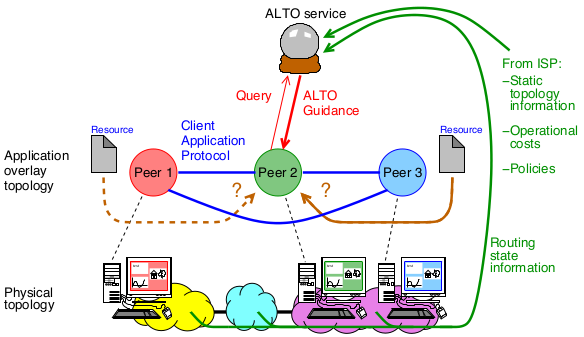
\includegraphics[scale=0.75]{alto-design.png}
    \caption{ALTO scenario \cite{seedorf2009}}
    \label{fig:alto-design}
    \end{figure}

        Despite its origins lying in the efforts to localize P2P applications, the ALTO protocol and encompassing system is now being considered in other fields, to be now further discussed.

        A first area of interest is CDNs, most specifically the current works in specifying the CDNI Request Routing Footprint \& Capabilities Advertisement interface \cite{alto-cdni(draft)}, which is a subset of the CDNI standard \cite{cdni-problem-statement} that aims to allow upstream CDNs to query known downstream CDNs if they are able and willing to accept the content request.
        In particular, one of the main functionalities of the CDNI request routing interface is the ability for upstream CDNs to retrieve static or dynamic information on download CDNs (resources, footprint, load), which they provide themselves, and that allow upstream CDNs to better choose the appropriate edge server that could serve a given end-user.
        ALTO serves as a good protocol to implement such functionality because it fits its use-case: some node (in the upstream CDN, where the content query originates) wishes to improve its routing (in regards to resolving content requests) by using information that is hard to deduce by itself to properly choose the most efficient node (the downstream CDNs where the content resides).
        At a more abstract level, this is similar to the use case fulfilled to P2P applications to help them better select peer connections.

        Edge computing, similarly to CDNs, use a paradigm of flexible service distribution that enables deployment closer to the end user for better performance, and thus is inherently effected by network status.
        Current work is being made on the benefits of using ALTO for the proliferation of network information to aid the task of deployment of functions or applications in the network edge \cite{alto-determining-service-edge(draft)}.
        Much like the previous example, ALTO is being used to guide an application in a decision with application and network resourcefulness impacts - by querying the ALTO server, the client can query for information that regards to points of presence (PoP) where functions/applications can be deployed, such as cloud computing provider's available resources, e.g., CPU, RAM, or storage, but also network information that pertains to the outside of the PoP, mainly network connectivity metrics, e.g., end-to-end bandwidth and delay, and routing costs.
        The utilization of the ALTO protocol in this context would allow edge service clients and providers, as well as ISPs, to combine efforts as a means to optimize edge computing deployment that considers the current network status, and doing so would thus result in benefits for both end-users and infrastructure maintainers.

        More broadly, current works are also being done in specifying abstract network entities path arrays between points \cite{alto-path-vector(draft)} and time-sensitive cost values \cite{alto-calendar-cost-map(draft)}, both of which share higher insight of the network, at the discretion of the ISP, as a means to provide even more context to applications about the infrastructure, such as identifying potential path bottlenecks and high traffic time peaks, respectively, and thus improve the ability of applications to properly generate application traffic on the network.

        A mode of operation where applications no longer operate in disregard to the network infrastructure they run on, but instead in deep consideration of it, could help significantly alleviate the issues emerging from the tension between the underlay and overlay, and is of mutual interest - improving application performance and reducing infrastructural costs.
        Enabling a communication channel can thus allow for many different co-operational use cases besides the aforementioned ones - for example, redirecting users to nearby data caches or warning them of server maintenance ahead of time.
        The existence of an all-encompassing oracle could also prove beneficial for applications which utilize periodic network probing to guide their choices, as such information could be measured by a select few nodes in the network and applicable to all nodes which are close-by to such node in ways that the ISP deems advantageous (such as belonging to the same AS or geographically near), thus minimizing the amount of probing used.
        ISP-guided counseling, however, does more than centralize measurements that could be done by the application itself - besides also containing measurements that could only be retrieved by the ISP due to its privileged access to the network (such as IGP packet inspections or secure SNMP queries), by handing over the decision-making process to it, the ISP is in position to better steer traffic in a way that favors internal policies, such as peering agreements, current traffic flow of other applications, known bottlenecks, etc, that could not be deduced by the applications alone.
        Thus, in the decision of how to generate application traffic, the responsibility should reside in both application and infrastructure as a way to benefit all relevant parties - the end users, the application stakeholders, and the service providers - and the ALTO protocol is an enabler of a mutually cooperative layer interaction mechanism that, by becoming the standard, would aid towards a sustainable life-cycle of the Internet.

        Finally, standardizing an architecture and related protocols for a clear problem domain could help a large subset of similar issues - a well defined and tested specification would exist, thus allowing many applications to leverage the ALTO protocol's functionalities to their needs, not requiring further cycles of development for a specification when one already exists.
        Also, the attempt to standardize the oracle pattern is helpful as it joins forces from many different domains which share common problems (many exemplified previously) into a single specification that interfaces with ISP knowledge, and would target issues such as security and scalability, creating a single point of convergence that is mature enough to be adopted by ISPs and applications, accelerating the transformation of the Internet as individual players would not need to develop their own specification.

    \subsection{Architecture}

        The high-level conceptual ALTO architecture can be seen on Figure \ref{fig:alto-architecture}.
        Central to the operation is the ALTO server, which stores network information and provides it to querying clients.
        Such network information is provided by trustworthy and relevant entities, such as information derived by routing protocols, ISP-specific policies, network historic measurements, and network feedback provided by third parties regarding application performance on the network.
        Two protocols can be seen as part of the general architecture: the provisioning protocol - not currently contemplated by the ALTO working group - should specify how information is provided to the ALTO Server; the ALTO protocol - main focus of the working group with the same name - specifies server-client interactions as a request-response interface for retrieval of network attributes.
        The ALTO client is the main consumer of the ALTO service as a whole, and it queries the ALTO server on network information whenever it deems such data as necessary to what it's doing at a given moment, with some potential use cases discussed previously.
        An ALTO client could be seen as any entity which is able to interface with the ALTO protocol with the role of a client, and as such is not tied to a specific implementation - in the example of P2P file sharing, a peer can act as an ALTO client (like the example scenario in Figure \ref{fig:alto-design}), but instead a tracker could enhance its role in assisting peer communication by having an embedded ALTO client which would then act on behalf of querying peers as to provide them with an optimal response, minimizing needed protocol modifications and thus facilitating integration with currently existing tracker-oriented P2P solutions.

    \begin{figure}[!t]
    \centering
    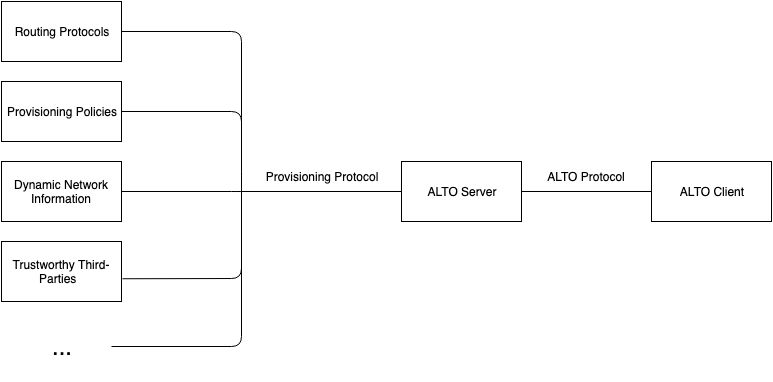
\includegraphics[scale=0.60]{alto-architecture.jpeg}
    \caption{ALTO architecture (adapted from \cite{alto-protocol}) }
    \label{fig:alto-architecture}
    \end{figure}

    \newpage

        The ALTO services contemplated by the corresponding working group can by visualized in Figure \ref{fig:alto-services}.

    \begin{figure}[!h]
    \centering
    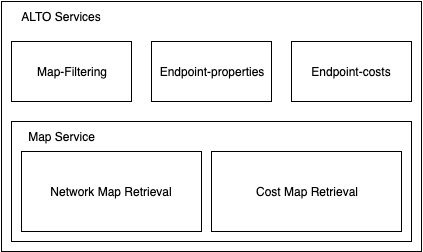
\includegraphics[scale=0.55]{alto-services.jpeg}
    \caption{ALTO services (adapted from \cite{alto-protocol}) }
    \label{fig:alto-services}
    \end{figure}

    The ALTO server stores and provides special mappings in the form of network and cost maps.

    A network map provides network location grouping identifiers and the corresponding aggregated endpoints.
    It utilizes Provider-Defined Identifiers (PIDs) as a key, and the mapping itself is left to the responsibility of the providers - it is thus a way of indicating that many endpoints should be handled similarly.
    A provider can then aggregate endpoints by geographical proximity, one or many subnets, one or many Autonomous Systems (ASs), etc., and attribute properties to the aggregate, instead of the endpoint.
    This is advantageous not only for scalability reasons - since it can compress information - but also because it allows ISPs to abstract network endpoints into groups, thus ensuring privacy of network topology details whilst maintaining useful network guidance, as the ISP has full control of how endpoints are aggregated, and consequentially how traffic is engineered since this changes how clients interpret resources.

    A second resource type provided is a cost map, which can be defined as a matrix M, where $M_{ij}$ - with i and j being the source and destination PIDs, respectively - is the associated path cost between the two indexes.
    The cost has two components: its metric and mode.
    The ALTO base protocol only defines a single, generic, cost metric called "routingcost".
    However, \cite{alto-metrics} is currently specifying more concrete metrics, with many associated with Quality of Service (QoS) evaluation, e.g., one way and round trip delay, packet loss and throughput.
    The other cost property, cost mode, can either specify that the metric is to be interpreted as a numerical value or as an ordinal ranking among all other costs in that cost map - this is useful in cases where too much network information is not deemed reasonable to share, and a simple order of preference that doesn't expose too much infrastructural detail can suffice.
    The decision to separate network and cost map information into two types of resources comes from the reasoning that network mappings are unlikely to change, whereas cost mappings could be periodically updated.
    As such, it alleviates client applications from the need to retrieve redundant information, and the ability to only retrieve a subset of it - this ability is further expanded in the map filtering service, which allows an ALTO client to further specify which regions of the requesting maps it wishes to retrieve (much like a "SELECT" statement from the Structured Query Language (SQL)), and only these are transmitted to it.

    Finally, the last two services focus on mappings that regard to specific endpoints, instead of abstract mappings that utilize PIDs.
    An endpoint is currently identified by one of the following: IP address, MAC address, or generic overlay ID.
    The endpoint property service maps to an endpoint a set of properties, e.g., geographical location or connectivity type, and the endpoint cost map has the same meaning of a cost map, but mapping to particular endpoints and not abstract collections.
    The ISP has thus the ability to work with abstract aggregates or specific endpoints, showing as little or as much network information as it deems fit.

    As could be seen, the ALTO project specifies an architecture for trading of network-related information, with well defined roles and a request-response protocol to fulfill interactions between them.
    It also attempts to standardize such interactions in the form of data structures with well defined attributes which are then to be manipulated for each use case.
    This could then serve as a useful service for any application that wishes to retrieve network information that could improve its decision making at the application level.
    It is important to note that there are restrictions to what kinds of information are contemplated by the ALTO protocol - for example, transport-level congestion is beyond its scope, and thus should not replace conventional mechanisms.
    The type of data which is valid to consider, according to \cite{alto-problem-statement}, should not be easily obtainable by the clients themselves (such as end-to-end delay), and should be variable on a longer timescale than the instantaneous kinds that are seen on, for example, congestion control mechanisms, as the frequently resulting querying traffic would be counterproductive to the task of traffic optimization.
    Potentially valuable information that is in the ALTO scope would then have to be harder to obtain without aid of this service, and not highly mutable through time - for example, routing costs, geographical locations, network proximity, operator's policies, scheduled down-times, etc.

    This project is, at time of writing, still on-working, with many drafts being created and updated, as the ALTO project matures and increased its domain applicability.
    These are, however, relating to service extension and deployment, since the main architecture, protocol design, implementation guidelines and security analysis are fully published into their respective RFC documents, serving as pillars for this work, and the ongoing efforts will serve as inspirations for potential extensibility.

\subsection{Viability}

\subsubsection{Security}
\label{sssec:alto-security}

    Given the nature of this system - the trading of sensitive network structure information that can alter application behavior - it is quite apparent that its design and implementation are not without challenges from a security perspective.
    \cite{alto-problem-statement} \cite{alto-protocol} \cite{alto-deployment-considerations} include discussions by the working group regarding security preoccupations at the development and deployment stages of the system.

    Utilizing the "STRIDE" threat model \todo{cite}, the main threats to the ALTO architecture can be summarized as follows:

\begin{itemize}
    \item Spoofing of a legitimate ALTO server that would mislead clients with wrong information - this could give the malicious party the ability to change traffic to its will.
        Spoofing of the clients themselves can also occur, and could allow a malicious party to retrieve sensitive network data outside their permission.
        Finally, spoofing of a provider of network status that could then feed information into the server to be spread into applications, possibly misleading them in the same way an ALTO server spoofing could, by proxy.
    \item Tampering of data to mislead either ALTO servers or clients.
        If some unauthorized and malicious party can retrieve data that is in transit or storage and tamper with it, clients would act on information that they assume is trustworthy but in fact has been modified.
        As such, clients could be redirected to wrong addresses, or receive incomplete or incorrect data that results in bad decision making.
        On the other hand, data tampering that occurs between data providers and the ALTO server would give it, a seemingly trustworthy party, untrustworthy data.
        This would result in the same issues that could arrive from spoofing threats.
        Tampering could also occur in input forms in the server-client or server-provider interface with potential to inject malicious code execution.
    \item Repudiation of being the source of some network information, whether it be by a third party that volunteered the data or the ALTO server itself, which would make it difficult to neutralize and attribute culpability to incorrect or malicious sources, jeopardizing the legitimacy of the provided network information .
    \item Information disclosure in the form of ALTO resources being made available to entities that were not contemplated to access it.
            These resources could give malicious parties insight on network topology status as well as the ability to derive clients' network usage patterns by observing what kinds of resources they attempted to retrieve in a given moment.
    \item Denial of service (DoS) of the ALTO server itself through query flooding beyond its capability, which would disable its ability to serve legitimate users.
        By proxy, service denial of external entities can also happen through the manipulation of ALTO resources themselves - leveraging the ALTO's potential to guide traffic, if a given resource is manipulated in such a way that unreasonable favors the preference of a specific subset of servers, these could be favourably picked by clients in a disproportionate matter, and highly affect these servers' availability.
    \item Elevation of privileges that lead to obtaining or modifying more information than initially permitted.
\end{itemize}

    Many of these threats are standard and could be solved with state of the art solutions which are well proven and tested, as indeed states \cite{alto-protocol}.
    However, threats of information disclosure - whilst they can be negated with in-transit encryption, what is done with this information the moment it reaches the client is hard to control - situations may arise when a client with proper resource permissions shares, intentionally or not, sensitive network information with one without, after interactions outside the ALTO architecture.
    Furthermore, many authenticated clients with different permissions could share information among themselves which they initially retrieved legitimately, to get a complete view of the network structure.
    Thus, individual clients could internally collaborate outside the system to bypass access control measures applied inside it.
    As such, it is firstly important for the ISP or third parties to carefully plan how what information they are comfortable with sharing, knowing that it may be susceptible to information disclosure outside the secure domain.
    Possible solutions to minimize these threats are as follows:

\begin{itemize}
    \item Reduce the granularity, and generally the details, of the provided data.
        Intuitively, the less granular and precise the shared information by the ALTO server is, the less valuable the resulting application guidance will be, and thus a balance would have to be found between layer cooperation and ISP privacy.
        One example is the usage of network groupings by PIDs instead of mapping information to concrete endpoints, working with network status around abstract entities.
        Another possible mean to reduce information granularity would be by utilizing ordinal cost values, which instead of specifying a concrete metric, e.g. bandwidth in bits per second or packet loss in percentage, the server would give a relative preference rating with lower costs meaning lower preference.
        In both examples, the granularity of network information transmitted to the client is several levels higher in abstraction than the actual physical layer, and this could reduce the flexibility of applications to optimize traffic.
        However, they can still provide acceptable flexibility without impacting ISP privacy, acting as a much needed compromise.

    \item Work only with a small set of trustworthy ALTO clients that are to act on behalf of a larger subset of less trustworthy clients.
        For example, network status resources could only be provided to authorized cooperation-oriented trackers in the BitTorrent protocol, which would in turn use this information to provide customized replies to clients without the need to change the base protocol.
        Similarly, information relevant for user-server assignment could only be provided to authenticated CDN control nodes, who'd share among them a private virtual domain to share information about user-server connectivity and server status that would otherwise be inappropriate for any other type of user.
        This is still, however, worthy of further threat analysis as restricted information could still leak outside of the system - beyond the means of spoofing discussed previously, seeing how a system behaves with ALTO guidance can give - albeit limited - insight into ISP bias.
        To see this, consider how a BitTorrent peer could continuously query a tracker with carefully crafted parameters - such as source address and candidate peers - and attempt to derive information from the resulting action, or similarly how a end-user could utilize similar parameter modification to observe the edge server selection mechanism in action.

    \item Utilize terms of agreements that are to be enforced on every querying client, stating that network status information does not get used beyond its original purpose, prohibiting sharing, and likewise that provided network information through third parties is not falsified.
        Although a potentially helpful mechanism to dissuade malicious users, it can be deemed impractical to apply, especially considering the scale at which this information could be shared.
        Thus, utilizing such means should be applied at a case-by-case situation and it should not replace ISP discretion and server resource maintenance to verify a given standard.
\end{itemize}

\subsubsection{Privacy}%

    Privacy concerns are also very prevalent in the ALTO system, being an ubiquitous talking point in most of the working group's problem statements and protocol specifications.
    When an ALTO client queries a server for one or more network status resources - in the attempt to optimize the application traffic it will generate in the near future - certain parameters can be passed to the server that can make the response be more personalized and contain more granular information.
    For example, a real-time P2P media-streaming application seeking ALTO guidance to help choose among a list of candidate streaming peers may wish to include in its query helpful parameters such as the peer list itself, the desired QoS metrics that should favor real-time media streaming, and the network position of the querying client itself.
    Indeed, these and more patterns will help increase the effectiveness of the ALTO server's guidance in helping the client application achieve its goal, but such happens at the expense of potentially allowing an ALTO server to infer on user pattern statistics.
    Even assuming that the previously discussed information disclosure threats are nonexistent in the ALTO system, privacy concerns can arrive from client applications because the resource queries they need to produce can contain information about what the client either will or wants to do.
    This is recognized by the ALTO working group as a possible concern \cite{alto-protocol} \cite{alto-problem-statement}.
    In response, they state that the clients should firstly be cognizant about the potential tracking risk that is associated with the usage of the system and, as an attempt to make tracking harder, they could disable HTTP cookies and/or opt for more vague query parameters, e.g. by randomizing some bits on endpoint addresses or simply using more broad addresses, whilst being aware that the helpfulness of query results may vary with increased parameter obfuscation.

    Privacy is likewise a concern towards the server side, as the ISP is providing sensitive network details to clients.
    Very much like client privacy, ISP-related privacy is also considered by the working group.
    Provider-Defined Identifiers (PIDs) were created as a means for ISPs to abstract network components as a collection of single network endpoints with similar properties, helping them not to disseminate network information that is too sensitive, and in turn also allows clients to make queries based on these identifiers and maintain a higher level of privacy.
    An ongoing proposal for protocol extension includes path vectors \cite{alto-path-vector(draft)}, that aim to represent information on the intermediary hops from a given source-destination pair, and each of these hops is represented as an Abstract Network Element (ANE) that, similar to PIDs, give ISPs the ability to under or over-abstract the topological representation that gets published to clients, giving more options to balance guidance usefulness with ISP privacy.
    Other solutions could also be considered depending on the needs of the clients and the direction of the project as a whole.
    For example, the servers themselves could operate on a secure communications channel and maintain a clear agreement on what can and cannot be made with the collected information.
    Alternatively, clients that wish not to impose much trust on the server's claims not to track them could make bulk queries (or use proxies to do so for them) and privately filter out the relevant information.

\subsubsection{Incentivisation}

    Incentivization relates to creating and divulging, to both layers, incentives to a fully cooperative layer relationship that is inherent in the oracle pattern adopted by the ALTO system.
    It is quite the challenge to fundamentally change how applications behave on the internet, as indeed it is to ask of ISPs to launch a view of their infrastructure to the outside world.
    \cite{dan-Commag10} notes incentivisation as one of the key challenges in overlay-underlay cooperation in regards to P2P applications, stating that incentive mechanisms need to exist to ensure that both layers both agree into and maintain a cooperative relationship.
    According to the ALTO problem statement \cite{alto-problem-statement}, the incentives for both parties to act on the system are the advantages that derive from using it - clients are to expect better application performance by leveraging ALTO guidance, and similarly ISPs should expect that their internal goals, such as an optimization of infrastructural utilization, can be met with the increased traffic engineering ability resulting from their oracle role.
    If the overlay consuming ALTO guidance has a manageable number of accountable entities - such as a single CDN or data center that the ISP agrees to partner with - it is realistic to maintain a cooperative agreement that can be solidified with feedback and service agreements.
    However, if the overlay utilizing the ALTO system makes it hard to pinpoint accountability, such as a large P2P application with many users, it will naturally be harder to ensure that the power dynamic between layers doesn't shift beyond an equilibrium.
    In these cases, policies should be created and enforced to give insurance to both parties that a cooperative relationship is maintained.

    The lack of cooperation could also occur by the ISPs, that could leverage their new-found application traffic engineering capabilities to steer traffic in a way that is advantageous to only them.
    Again, much like the lack of cooperation by clients, it is difficult to guarantee an equilibrium in the power dynamic between layers, but by guaranteeing improved QoS levels for applications that utilize ALTO cooperation, ISPs become responsible in guaranteeing that these improvements are met, fearing client abandonment otherwise.
    Giving freedom to both layers on how they act ensures that the system evolves to a common ground that benefits both sides, at least enough to justify them remaining there.

    Finally, if the application-ISP tussle becomes harsher, as it tends to, a cooperative system such as ALTO may become necessary - and thus beyond preferable - meaning that ISP may be forced to block or throttle traffic that it cannot route properly, as it historically happened.
    Thus, acting with ALTO goes beyond cooperation into symbiosis, meaning that both parties have to act cooperatively to maintain network sustainability.
    Regardless, the best approach seems to be that the system must in of itself be self-justifiable, meaning that the advantages that it brings should be enough to convince both parties to act on it.
    ISPs are nevertheless free to deploy their own incentive mechanisms to facilitate early application adoption, that could include monetary rewards or routing privileges.

\subsubsection{Network Neutrality}
    As stated by \cite{qos-framework}: "According to most network neutrality proponents, network neutrality rules are intended to preserve the Internet's ability to serve as an open, general-purpose infrastructure that provides value to society over time in various economic and non-economic ways. In particular, network neutrality rules aim to foster innovation in applications, protect users' ability to choose how they want to use the network, without interference from network providers, and preserve the Internet's ability to improve democratic discourse, facilitate political organization and action and to provide a decentralized environment for social, cultural and political interaction in which anyone can participate.".
    Network neutrality has been a popular point of discussion as society grows around the Internet, sparking debates around the world on what the best course of action should be - for example, regulations were introduced by the FCC in the United States \cite{fcc} to police network neutrality, and the European Union has a framework for net neutrality laid down by article 3 \cite{article-3}.
    However, potential violators of the spirit of a network neutrality exist, such as British Plusnet's usage of deep packet inspection (DPI) to implement limits and differential charges for different traffic \cite{arstechnica}, or Portuguese MEO's smartphone contracts which include zero rating programs for a given set of services \cite{meo-packages} that bundle applications such as Facebook or Spotify.
    Network neutrality advocates are concerned with guaranteeing that ISPs keep Internet communications free and do not discriminate based on the traffic's specifics, such as platforms, applications, or source and destination.
    On the other hand, opponents of net neutrality, among them ISPs, broadband and telecom companies, and hardware manufactures, argue against net neutrality - they claim that it would would reduce incentive to invest, as investments would be harder to insure without the ability to charge higher rates for better infrastructure capabilities.
    Zero rating programs, such as Wikipedia Zero, which provides Wikipedia with no charge to a select group of low income regions \todo{cite} , would also not be possible.
    Additionally, with net neutrality, the ISP's ability to route traffic could itself be at jeopardy - as \cite{jerzy} states in their solution to compromise net neutrality with QoS demands via service differentiation, the Internet is growing at an astonishing rate, as are the QoS demands of applications, and operating the infrastructure on a purely best-effort basis will not be sufficient without a constant provisioning of such infrastructure to keep up with demand, and this too may not be viable nor even possible.
    Thus, discriminating by traffic services may be needed to guarantee that, say, real-time medical information gets priority over real-time media streaming, which in turn gets priority over e-mail or file sharing.

    Considering that the ALTO system behaves in an oracle pattern of cooperation where a single entity - the ISP - is able to heavily influence the traffic patterns of the applications it aids, on the promise of a cooperative network underlay-overlay relationship, such system could violate the principles of net neutrality.
    In particular, this could happen if the oracle either blocks, or at the very least provides different guidance to different clients, depending on where the query originated from - e.g. what application, source address, or other defining characteristics.
    A possible consequence of such a system guiding the Internet could be that given applications can consistently have better QoS measurements not on the basis of the application's implementation, but on the ISP personal biases.
    Oracle systems such as ALTO do not seem to be analogous to other traffic engineering strategies, such as the usage of MPLS, DiffServ, nor to other means of ISP intervention on overlays, such as the deployment of data caches and redirector proxies - this is because the oracle system, in contrast to the previously mentioned strategies, is one of mutual voluntariness and cooperativeness between ISPs and applications.
    However, it could be argued that if the ALTO system offered guidance to applications in such a way that consistently resulted in better application performance, such applications would be pressured to use such guidance as a means to remain competitively viable, and the ISPs would then have a platform to influence a considerable amount of traffic to their will, being in a position to, depending on how they treat guidance requests, break network neutrality.
    This neutrality concern can be alleviated if application guidance operated on classes of traffic, e.g. real-time communication or file sharing, thus operating on traffic aggregates to insure QoS levels needed to given application types, but never discriminating beyond such given classes.

    As the protocol is defined \cite{alto-protocol}, the provided network status information is truthful and guidance is optional, and neutrality can then still remain outside of the system, since no routing measurements exist within it.
    If particular implementations of the ALTO system give guidance in such a way to guide traffic in a discriminate fashion, and if such guidance have advantages that much outweigh any alternative - thus rendering it beyond optional - a case can be made for how ALTO as a concept can break network neutrality - for all its advantages and disadvantages discussed bellow - as the ISP can utilize discriminatory behaviour to treat applications on their infrastructure differently.

\subsubsection{Multi-Domain orchestration}

    The Internet as we know it today spans the entire globe and is rather complex in nature.
    According to \cite{dan-Commag10}, the classic vision of the Internet consisting of a network of transit and stub ASs no longer seems accurate, as it now is much more complex - for starters, the role of network owner and service provider are separating, and Internet access is provided by numerous competing ISPs.
    As a demonstration of such complexity, Figure \ref{network-connectivity-globe} displays how the Internet is structured into many tiers of different service providers.
    It can thus be seen that the act of layer cooperation can get harder when the influence domain increases and potentially spans many different ISP regions which will inevitably act differently as they can have different technologies, biases, policies, and overall goals.
    These per-ISP biases can make it difficult to guarantee that traffic optimization spanning multiple administrative domains is actually useful and achieves the cooperative nature in mind - for example, an ISP may not be comfortable categorising end-point costs of a given metric, thus making path calculations that pass through that ISP domain not viable.
    Regardless, per-domain ISP guidance has nonetheless plenty of potential - for example, the ability to localize traffic, as entities outside of domain can be identified by ISP, and similarly per-domain optimization of resources can still be useful when such domain is large, and can be applied to high-volume operations such as those in a data center.
    The ALTO server within a given domain can also leverage probing measurements and feedback statistics to derive information in areas whose topological detail is unknown, giving a partial network view that contains topological insight and also information derivation that, whilst not being as good as a complete topological insight, may nonetheless power a cooperative effort within a given domain with good results.
    Some data may, whoever, be both not shared by an external domain nor derivable - endpoint property information, such as network connection types, or server footprints - e.g., available cpu, ram and storage - can only be retrieved by authoritative entities in a given domain and probing to them may be not available, thus considerably limiting the applicability of a single ALTO domain.

    \begin{figure}[ht]
    \centering
    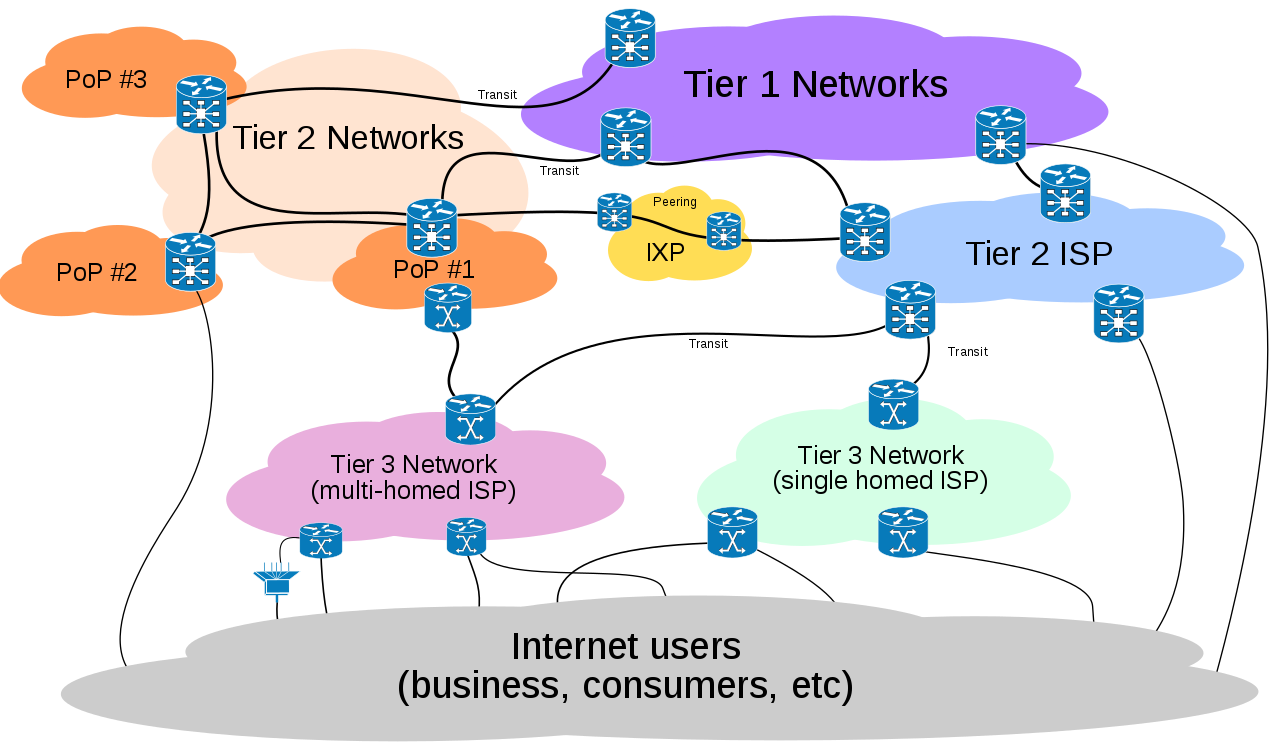
\includegraphics[scale=0.30]{network-connectivity-globe.png}
    \caption{Conceptual representation of ISP diversity on the Internet}
    \label{fig:network-connectivity-globe}
    \end{figure}

    Even assuming that all ISPs are comfortable with sharing sufficient information, ambiguity may arise - considering a cost map with the generic "routingcost" cost metric, ISPs could internally calculate routing costs differently, and prioritizing different goals, e.g. reducing overall link usage versus reducing inter-AS traffic first and foremost.
    The base ALTO protocol specification states that each network region can provide its ALTO services, which in turn convey network information from their perspective.
    A network region consists of a given administrative domain, such as an AS, an ISP, or a given set of agreeing ISPs \cite{alto-protocol}, thus implying that if multiple ISPs share an ALTO server they must reach a consensus on what network status is available for query from the outside.
    Furthermost, the ALTO working group's deployment considerations \cite{alto-deployment-considerations} document states that an ALTO client can query a single server for one or many metrics, or he can additionally query multiple server instances on different networks \cite{alto-deployment-considerations}.
    It is explicitly stated in the document that each server could give guidance for only a given network partition, and such guidance may wildly differ between them due to the fact that different algorithms and objectives may have been applied.
    The document also states that, in regards to extending ALTO's reachability, three different strategies could be applied:

\begin{itemize}
    \item \textbf{Authoritative Servers}: A given set of servers can provide guidance for all kinds of destinations to all ALTO clients.
    \item \textbf{Cascaded Servers}: An ALTO server can possess an embedded ALTO client and query other ALTO servers if it cannot serve the original request, acting as a middleman between the client and the more apt server.
    \item \textbf{Inter-server Synchronization}: Different ALTO Servers communicate among themselves to expand the knowledge space.
\end{itemize}

    The last strategy is still being subject to development and standardization by the working group as part of a bigger attempt to link different network regions and technologies into a single, homogeneous abstraction of the Internet.
    Current efforts in multi domain orchestration and relevant use case examples are summarized in the ongoing work of \cite{ALTO-multi-domain-use-cases(draft)}.

\section{Summary}

\todo{Finish this}

\textbf{[Mention how in all overviewed cases (p2p, cdn, client-server) there is something to be gained on both sides by enabling layer cooperation. By better knowing how the network is structured, better application decisions can be made that minimize network resources, and this in turn is also befinitial for ISPs. All the seen cases suffer in how to better match given entities that wish to generate traffic, whether that be between peers, between edge clients and edge servers, or between clients and server replicas, respectively. ALTO's usefulness goes beyond this, and also provides a standardized means through which a centralized, well maintained  framework helps retrieve network status and ISP influence to increase application awareness. This helps, for example, not only to better select between redundant service entities, as seen before, but also to better decide when to perform a given network action in accordance to the current network status, how to select new and appropriate nodes to the application, how to extend the domain knowledge of the network, etc.]}
